\documentclass[man,floatsintext]{apa6}
\usepackage[utf8]{inputenc}
\usepackage{amsmath}
\usepackage{amsfonts}
\usepackage{amssymb}
\usepackage{apacite}
\usepackage{rotating}
\usepackage{array}
\usepackage{multirow}
\usepackage[table]{xcolor}% http://ctan.org/pkg/xcolor
\usepackage{graphicx}
\usepackage{todonotes}
\usepackage{caption}
\usepackage{subcaption}
\usepackage{url}
\usepackage{slashbox}
\newcommand{\co}{\cellcolor{gray!40}}

\title{Robots Showing Emotions: Emotion Representation with no bio-inspired Body}
\author{Julian M. Angel-Fernandez and Andrea Bonarini}
\affiliation{Department of Electronics, Information, and Bioengineering\\ Politecnico di Milano\\ Milan, Italy\\
email: \{julianmauricio.angel,andrea.bonarini\}@polimi.it}

\abstract{Robots should be able to represent emotional states to interact with people as social agents. There are cases where robots cannot have bio-inspired bodies, for instance because the task to be performed requires a special shape, as in the case of home cleaners, package carriers, and many others. In these cases, emotional states have to be represented by exploiting movements of the body. In this paper, we present a set of case studies aimed at identifying specific values to convey emotion trough changes in linear and angular velocities, which might be applied on different non-anthropomorphic bodies. This work originates from some of the most considered emotion expression theories and from emotion coding for people. We show that people can recognize some emotional expressions better than others, and we propose some directions to express emotions exploiting only bio-neutral movement.
}

\shorttitle{Robots Showing Emotions}

\begin{document}
\maketitle
\section{Introduction}
The expression of emotion in robots is becoming a quite important issue to implement robots able to interact with people in a social context. Following the results obtained by studying emotion expression in humans (e.g., \cite{Venture2014,Ekman2004}), it is possible to notice that most works focus on facial expressions (e.g.,~\cite{Breazeal2002}) or on humanoid poses (e.g.,~\cite{Canamero2010}), while the vast majority of robots on the market nowadays are not provided with face, arms and legs. Moreover, the focus is often on the position of limbs, or face elements, more than on the kind of movement that could express emotion, resulting on emotion expressions that could not be broadly used in most platforms.
There are applications where the shape of the robot is constrained by functional needs, such as in the case of home cleaners, lawn mowers, transporters, flying drones, and many others. In all these cases, emotions can be expressed with the only available body, exploiting movement features.

The work presented in this paper focuses on the identification of movement features that could be considered platform independent, thus could be used to express emotions with a wide range of robots. We devised a very simple robot base, with no resemblance to humans or animals, and we proposed its movements to subjects, to identify how they could interpret the movements they could see from a robot in front of them. We performed live trials to keep into consideration factors that could influence the evaluation: the full perception of movement and noise, and the interaction with a physical robot are different if the same scene is lived in first person, or seen on a screen as a movie.

The obtained results enable to say that it is possible to design movements, even for a neutral platform, that could be interpreted as emotional expression, with some differences among emotions, as confirmed also by other experiments in robotics~\cite{Sharma2013} and suggested by psychologist~\cite{Russell2003}.

Finally, we could identify a set of very basic movement features that could be used to express emotions and, most importantly, the range of values for these features that could led to successful implementations.

This paper is organized as follows. The next section provides a brief overview of relevant work related to emotion expression in robots. Section~\ref{sec:robotic_platform} outlines the platform used in the case studies. Section~\ref{sec:cases} presents the design and results for all four case studies.
\section{Related Work}
\label{sec:related_work}

It is not possible to apply a direct mapping from human studies to robots~\cite{Saerbeck2007,Canamero2010}. Nevertheless works done in human studies provide guidelines about possible features and values that could be used to generate emotional motion. 

\subsection{Human Studies}

Emotion plays an important role in human-human interaction and can be expressed through diverse channels such as body gestures and poses, body movements, face expressions. The human face is a complex structure that embraces more than 43 muscles act. Hence, the face has been considered as a primary channel to express emotion. As a consequence, many works have focused on facial expression, mainly but not only, influenced by the work done by Ekman~\cite{Ekman2004}. However, the role that body plays in emotion projection has been recognized and it has been started to be studied~\cite{Gelder2008,Wallboot1998}. Nevertheless, the amount of works related to body expression of emotions is still small compared to studies about facial expression. 

Analysing some of the few works that have studied human body expressiveness, it is possible to recognize two different methodologies to create the data base of movements to be assessed during the experiments. The first methodology uses human actors (either professionals or amateurs) to walk straight from point A to point B conveying specific emotions~\cite{Dael2012,Meijer1989,Wallboot1998}. Each trial is recorded and later shown to each subjects that have to classify all the sequences. The second methodology uses virtual agents~\cite{Roether2009,Venture2014} to generate the very same set up for the experiments; the agent's movements are generated from the data recorded from human actors.

The work done by Wallboot~\cite{Wallboot1998} has been used as a reference by other researches. It addressed the question: \textit{Are specific body postures indicative of emotion or are they only used to indicate the intensity of the emotion?} To answer this question, he recorded 224 videos for joy, happiness, sadness, despair, fear, terror, coldness anger, hot anger, disgust, contempt, shame, guilt, pride, and boredom, and showed them to the subjects. His results reaffirm that movement and body postures are indicative of intensity for some emotions. But at the same time, these two characteristics seem to be enough to identify other emotions. 

Complementary studies using virtual agents have been performed by  Kluwer and collaborators~\cite{Kluwer2004}, who studied the contribution of postures and angle view in the interpretation of emotions. They generated 176 static positions for happiness, anger, disgust, fear, sadness and surprise. Each image was later rendered from three different angles (front, left, and above and behind left shoulder) producing a total of 528 images. All the participants were exposed to all 528 images and were asked to label the image with the emotions that best represent it. Their results show that five out of six emotions were quite well recognized independently from the angle of view., while disgust was for some postures confused with fear.

There are two main drawbacks of all these projects that use video recorded sequences. First, they miss the impact related to a complete physical experience. For instance, it is clearly different facing an angry robot really rushing against us, or looking at a video where this happens. Second, each actor has his/her own way to represent a given emotion~\cite{Russell2003,Gunes2011}. Actors use diverse techniques to create believable representations of specific emotions. However, this does not ensure that all actor convey emotions in same way. Therefore, several records are done and the ones with the highest agreement are selected. This brings the technical question on how to interpret the significance of agreement obtained~\cite{Russell2003}.

\subsection{Robotic Studies}
%%%%%%%%%%%%%%%%%%%%%%
As a direct consequence of the abundance of works in face elicitation in humans, most of the works done in Human-Robot Interaction (HRI) have focused also on faces. One of the most well-known expressive robots is Kismet~\cite{Breazeal2002}, a robotic face able to interact with people and to show emotions. The face had enough degrees of freedom to portray the basic emotions suggested by Ekman~\cite{Ekman2004} (happiness, surprise, anger, disgust, fear, and sadness), plus interest. 
Despite the complex system behind Kismet, the emotion's projection evaluation was done using videos with a very limited number of participants. Similar approach was followed by Li and Chignell~\cite{Li2011}, who used videos of a teddy bear robot to study the contribution of arms and head movement to express emotions. In same direction Destephe and collaborators~\cite{Destephe2013b,Destephe2013} studied the attribution of emotion to a robot's gait using a virtual representation of the platform WABIAN-2R. More recently Knight and Simmons~\cite{knight2016} used Keepon and NAO platforms to study the possibility to project inner states with just head movements. Although use of videos has the advantage to cover a major number of participants, the lack of interaction with the real platform make these works lose the impact that a robot could generate on the participants.  

%%%%%%%%%%%%%%%%%%%%%%%%
The use of real platforms to study emotion projection could be dived in two lines: using anthropomorphic and non-anthropomorphic platforms. In the first case, these works are characterized by the use of cue positions to project desire emotions~\cite{NAO2013}. In some cases, special attention has been taken to determine head's angle and arms position contribution in specific emotions~\cite{Brown2014}. 
Nevertheless, current humanoid platforms cannot generate smooth gaits, which limit the study of body movements. For example Karg et al.~\cite{Karg2010} tried to map actors gaits on an hexadop robot to understand the contribution of step length, height and velocity. Their results suggest that using this approach is not suitable because the difference between different gaits are not recognizable. So they suggest that movements must be exagereted.  Some researchers have reduced the human appearance (e.g. eliminating limps and facial expressions)to increase platform mobility and study new mechanisms to project emotions~\cite{Arras2012}. Pushing forward the reduction on anthropomorphic features, Saerbeck and Christoph used a Roomba platform to study the contribution of curvature in a trajectory to conceive emotional states~\cite{Saerbeck2010}. Similarly Lourens and Barakova~\cite{BarakovaL10} implemented a set of behaviors to determine the emotion  perceived from diverse movements, which were selected from the  work done by Camurri et al.~\cite{pop00002}. Continuing with her research on how robotics' behaviours are interpreted by people, Barakova and collaborators~\cite{Barakova2013} created a closet in which lights could be manipulated to convey pre-defined behaviours. The robot's behaviours were defined using the Interpersonal Behaviour Circle (ICB)~\cite{Leary57}, which is based on two dimensions (dominance-submission and hate-love). Their findings suggest that electronic systems can elicit a type of reactions different from the one expected by theories of interpersonal communication.

Other approaches have tried to get a better understanding of the contribution of diverse features to express emotions through movement. For example, Suk and collaborators payed a particular attention to speed, smoothness, granularity of movement path and volume of a non-bioinspired object~\cite{NAM2014}. They used the self-assessment (SAM)~\cite{Lang2008} method to evaluate participants. Their results suggest that arousal increases as speed increases and that there is not any clear tendency for smoothness. On the other hand, granularity is positively correlated with pleasure and arousal, while volume is negatively correlated with pleasure and positively correlated with arousal. Alike, Tan and collaborators~\cite{Tan2016} have studied the contribution of velocity, fluidity, direction and orientation of a small box. They evaluated participants' perception using SAM. Their results suggest that direction is directly correlated with dominance, but that fluidity does not influence the perception. While flat orientation is related to positive valence, leaning position are related with negative valance. Finally the velocity is correlated with valence, arousal and dominance. Using an hexapod robot, Karg et al. studied 

Due to the popularity that quadrocoptors have received in the last years, Sharma and collaborators~\cite{Sharma2013} used a quadrotor to study how different Laban's effort~\cite{Laban1968} parameters could impact on the perception of affection. A professional Laban certified actor was asked to generate 16 different paths, for each one changing one of the four Laban's parameters (space, weight, time, and flow). Each generated path was recorded using the Vicon motion-tracking system. Continuing with the use of quadrocoptors, Cauchard and collaborators~\cite{Cauchard2016} studied how flight paths could project personal traits and emotional attributes. All these works present a very nice starting to point to identify features and values that could be used to project emotions in robotics, which could help in coordinating humans and robots~\cite{Novika2015}. However, all of these works not give a price guideline to elicit precise emotions, which from our previous case studies could lead to the misinterpretation of movements emotions~\cite{Angel2016}. For example people could confuse an implementation of \textit{Happiness} with \textit{Anger}.
\section{System}
\label{sec:robotic_platform}
The system used in the case studies here reported has been developed to support the identification of features that could be used to project emotions with a non-bio-inspired platform. This system is composed of two complementary parts: robotic platform and emotional enrichment system. The platform has been envisioned to be as simple as possible without any resemblance to anthropomorphic embodiment, while the emotional enrichment has been designed to be applied also to other platforms and to be extended to other emotion expressions.
 
\subsection{Robotic Platform}
The platform is a holonomic base, as shown in Figure~\ref{fig:holonomic-platform}. The first prototype included three metal gear motors with encoders, an Arduino Mega micro-controller, one servo motor and X-Bee system to enable the communication between Arduino and a remote computer. The mechanical design of the prototype is shown in Figure~\ref{fig:triskar-prototype}. A PID controller for each wheel was implemented and tuned to guarantee the desired linear and angular velocity.

This prototype was modified after the first experiments to improve the expressiveness of the upper part. Two additional servo motors and a mechanical structure to support all these motors were added. The two motors attached to beams could be controlled to obtain an asymmetric or opening-closing movement. 
The third motor deforms the upper part of the foam. Figure~\ref{fig:triskar-first-design} shows the placement of the motors. To hide the structure, foam and a light blue cloth covering the foam were used, as it could be seen in Figure~\ref{fig:triskar-cover}. The light blue color was selected because it is not expected to generate any particular arousal in people~\cite{Naz2012}. 

Although this version showed the possibility to convey emotions, still it was not autonomous enough to host the emotional enrichment system. Therefore, an Odroid-U3 microcomputer was added, communicating with Arduino Mega via ROS-Serial.
Also, it was decided to make some improvements in the upper part. Two reasons motivated these changes. First the deformation system was not changing the shape enough to be clearly perceived by subjects; second, the beams were damaging the foam. Therefore, a lever was added to the deformation motor, and a piece of rubber was adopted to safely connect the beams with the foam. The final arrangement is shown in Figure~\ref{fig:triskar-second-design}.
 
The final version, with improved computational power (Arduino Due instead of Mega) is shown in Figure~\ref{fig:triskar-third-design}.
\begin{figure}[h]
	\centering
	\begin{subfigure}[c]{0.3\textwidth}
	\centering
	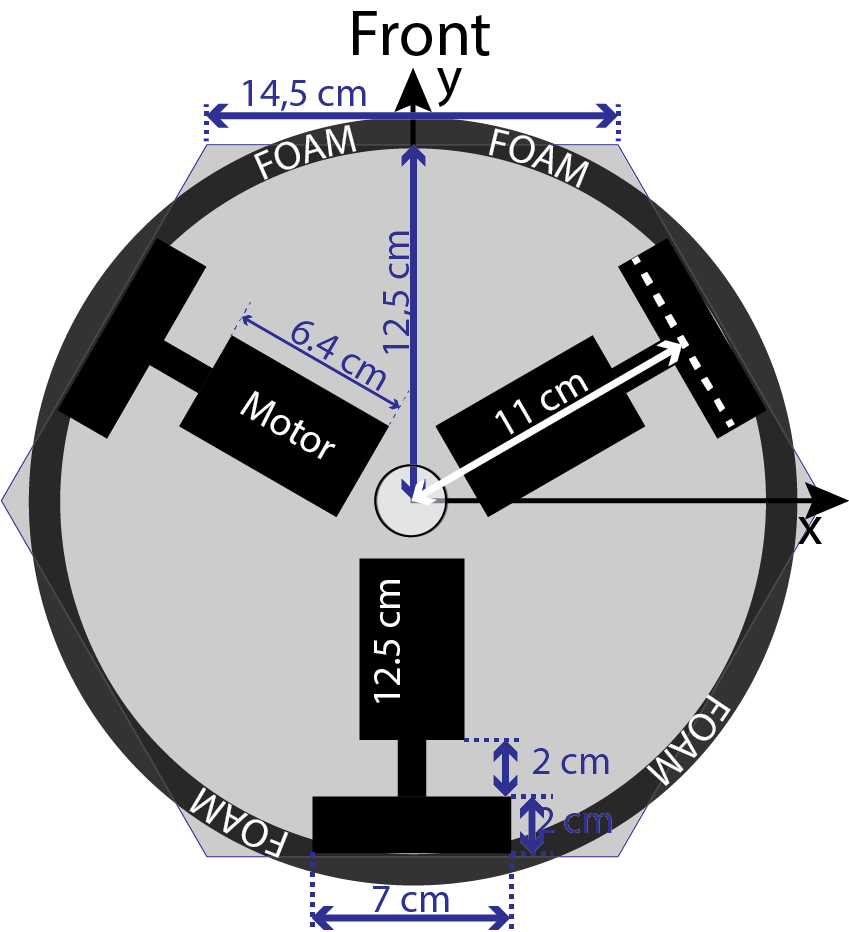
\includegraphics[width=\textwidth]{./Images/TriskarThird.png}
	\caption{Holonomic Base used in all the platform's version.}
	\label{fig:holonomic-platform}
	\end{subfigure}
	\begin{subfigure}[c]{0.3\textwidth}
	\centering
	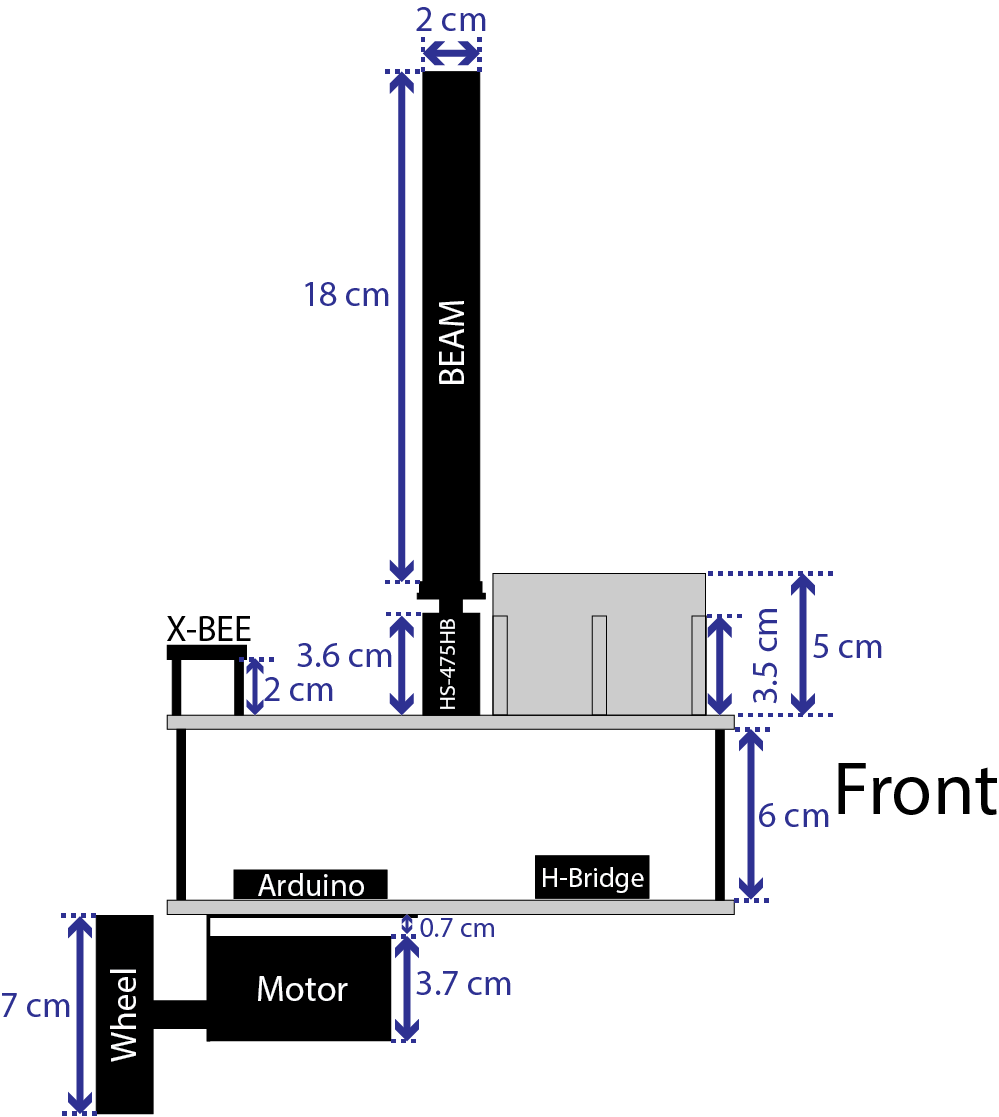
\includegraphics[width=\textwidth]{./Images/upperFirstB.png}
	\caption{Platform prototype.}
	\label{fig:triskar-prototype}
	\end{subfigure}
	\begin{subfigure}[c]{0.3\textwidth}
	\centering
	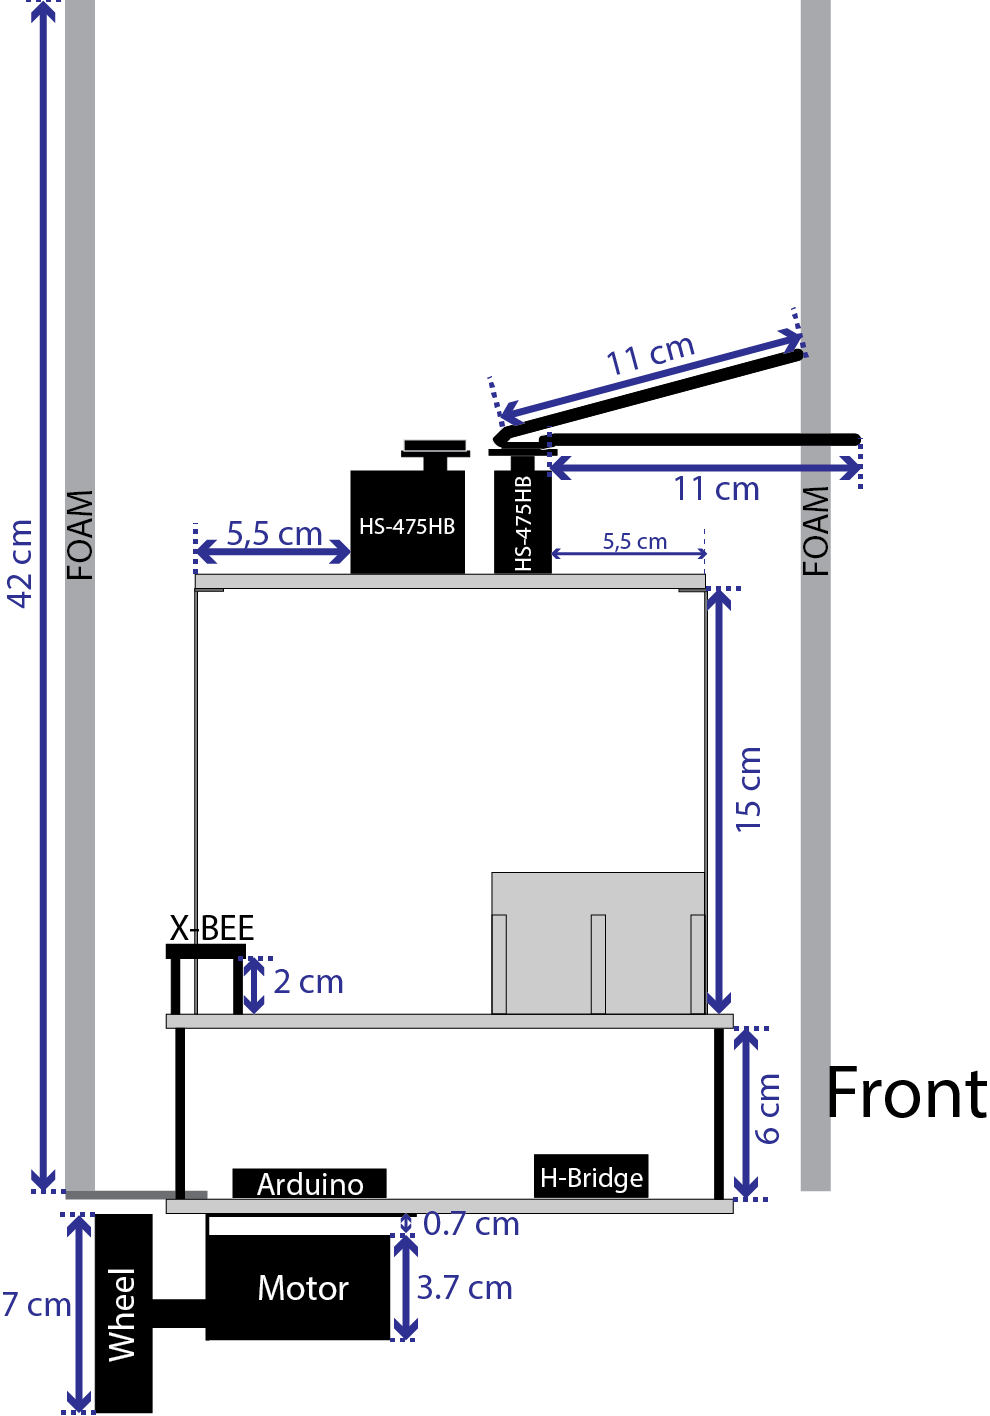
\includegraphics[width=\textwidth]{./Images/upperSecondC.png}
	\caption{First version design.}
	\label{fig:triskar-first-design}
	\end{subfigure}
	\\
	\begin{subfigure}[c]{0.3\textwidth}
	\centering
	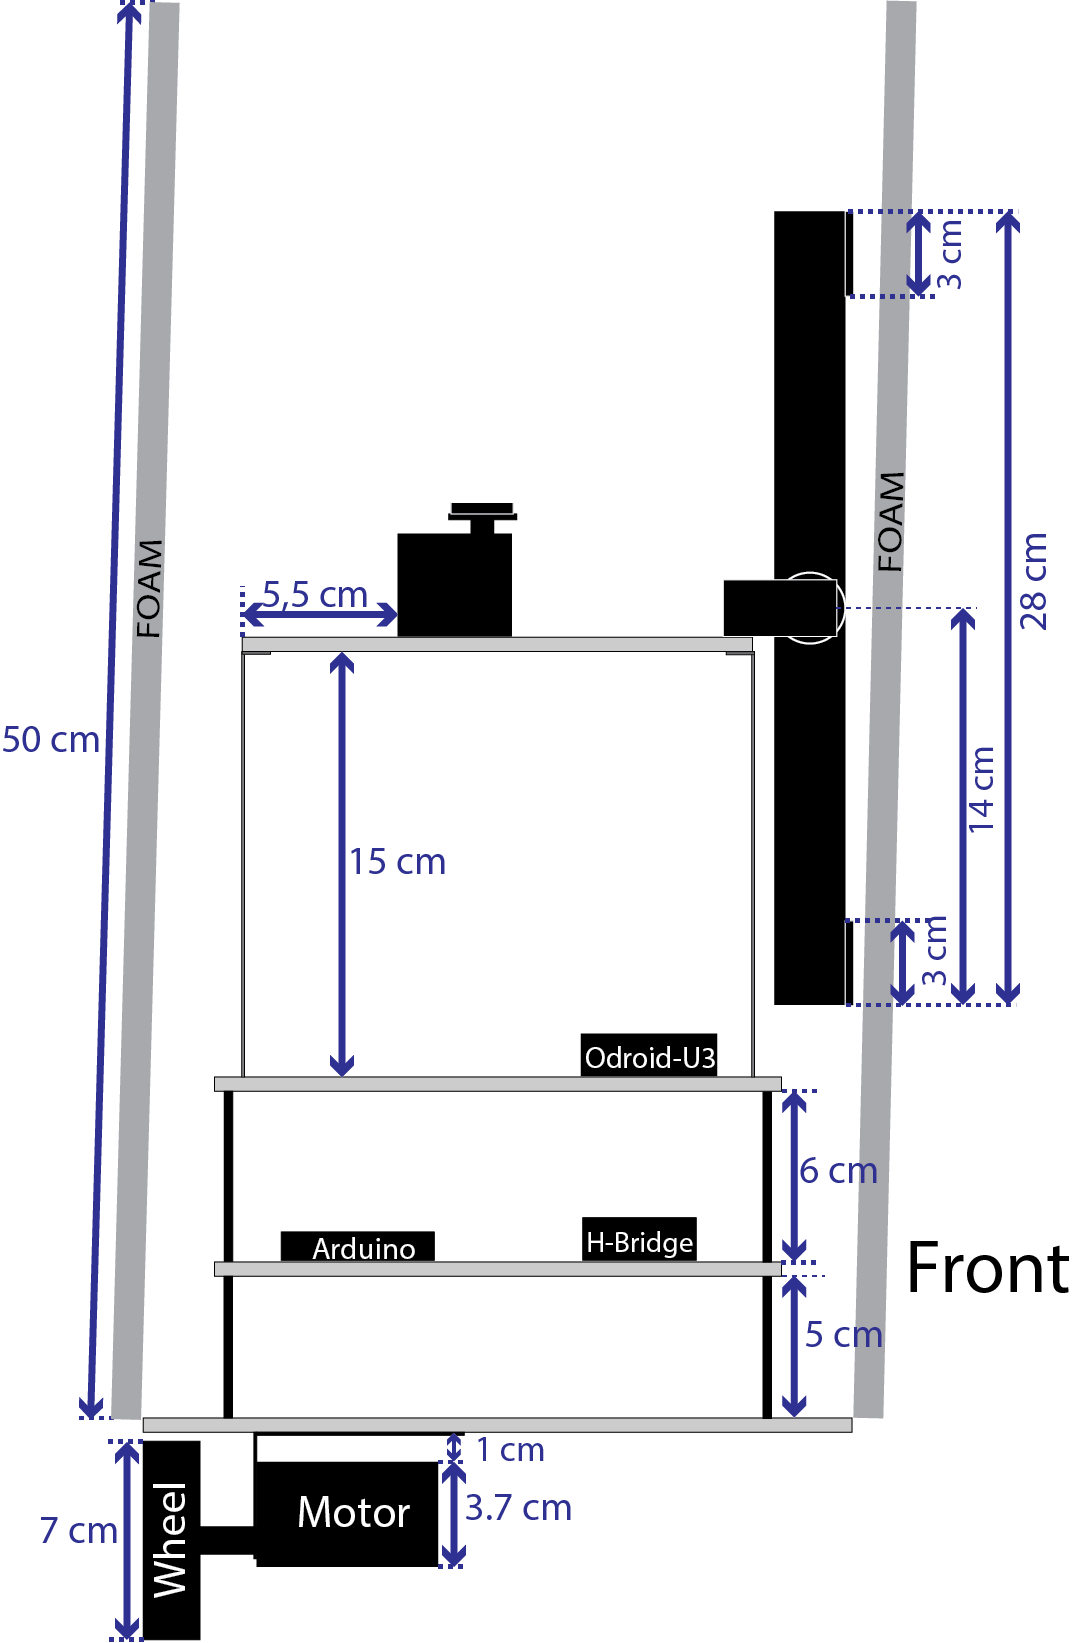
\includegraphics[width=\textwidth]{./Images/upperThirdD.png}
	\caption{Second version design.}
	\label{fig:triskar-second-design}
	\end{subfigure}
	\begin{subfigure}[c]{0.3\textwidth}
	\centering
	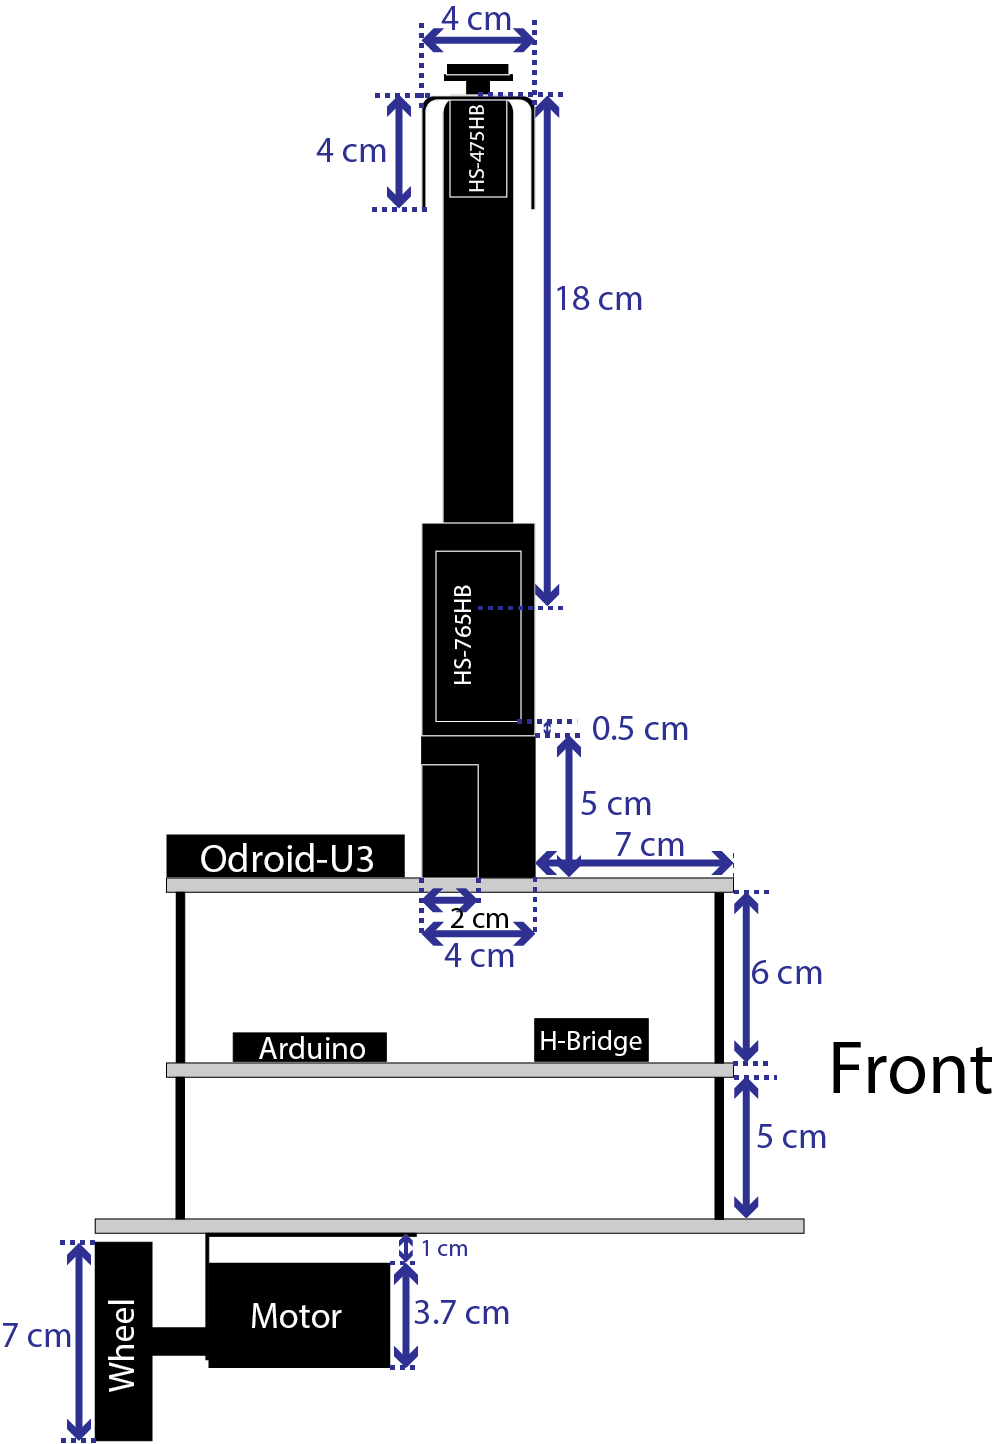
\includegraphics[width=\textwidth]{./Images/upperFourthD.png}
	\caption{Third version design.}
	\label{fig:triskar-third-design}
	\end{subfigure}
	\begin{subfigure}[c]{0.3\textwidth}
	\centering
	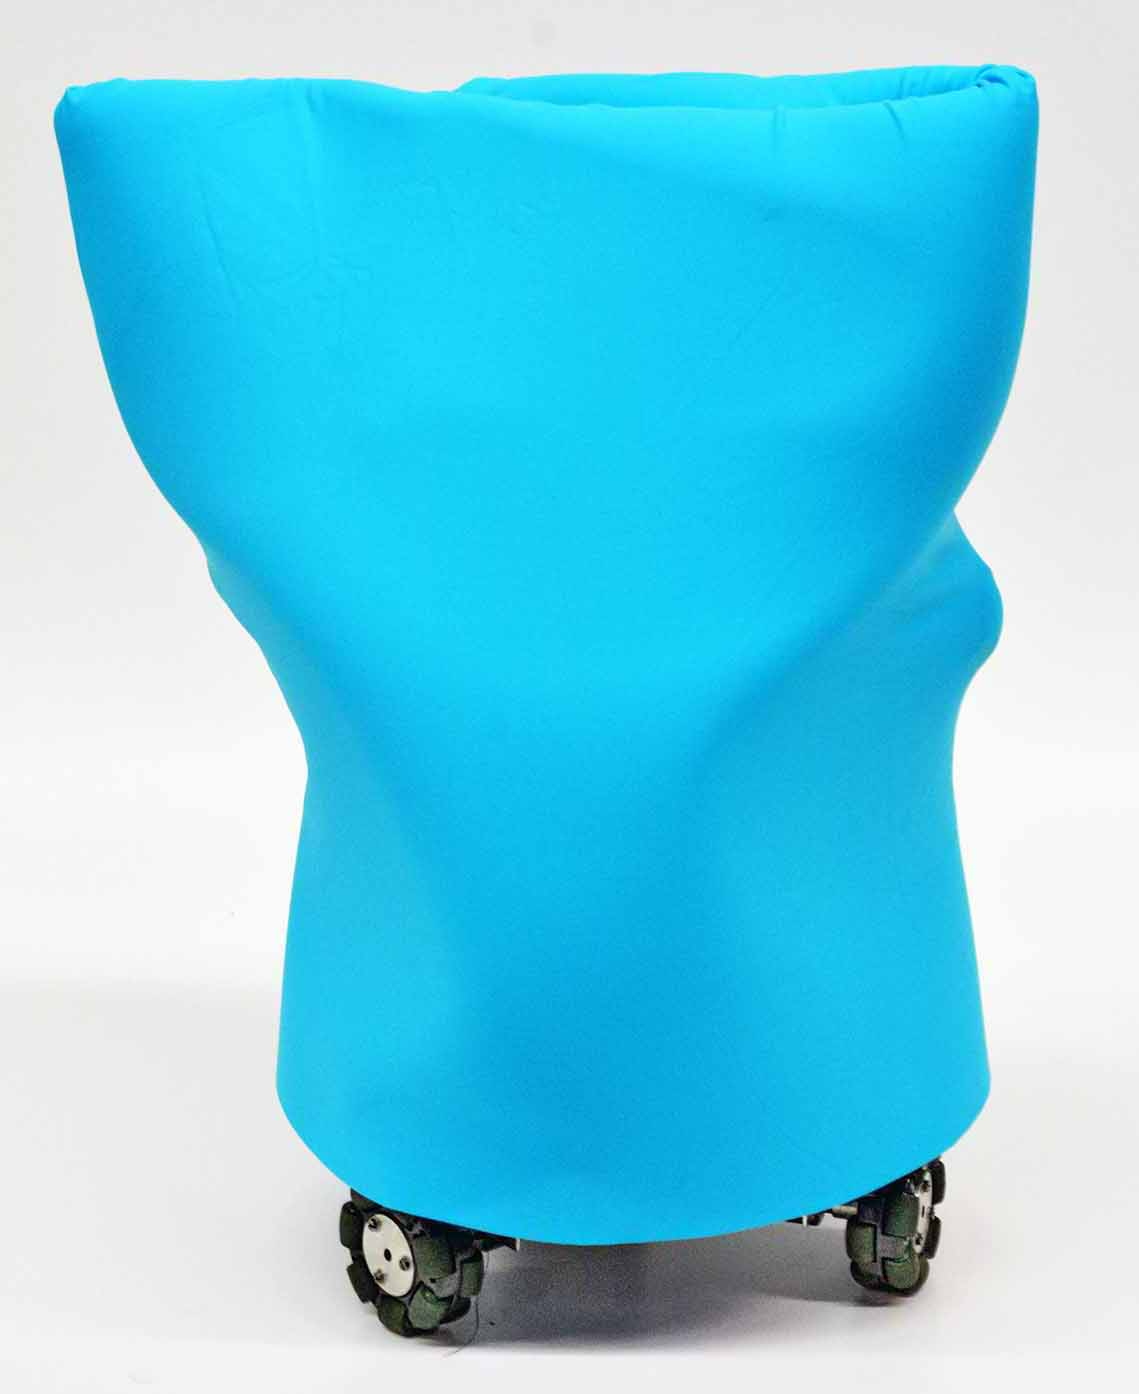
\includegraphics[width=\textwidth]{./Images/Triskar2.jpg}
	\caption{Platform with cover.}
	\label{fig:triskar-cover}
	\end{subfigure}
	\caption{Triskarino platform.}
	\label{fig:robot}
\end{figure} 
\section{Case Studies}
\label{sec:cases}
In total, we did one pilot and four case studies using changes in linear and angular velocity, and oscillation angle to convey emotions. These features are depicted in Figure~\ref{fig:features}. The pilot was used to test the prototype and identify possible improvements. The feature values for the first case study were selected empirically and robot's movements were presented to participants. The results suggested that it was possible to convey some emotions, but it was decided to give a context to each emotion to test whether this could increase the recognition rate. A second case study was designed. Each emotion was presented to the participants in a context of a small scene, which was portrayed by the robot and a non-professional human actor. The results suggested that showing the emotion in a context can improve the recognition of some emotions, so that the robotic emotional expression could be at least perceived as coherent with the context. However, the study of the impact of the actor and context were not in the aims of this research. To compare with literature on emotion projection, a third case study was implemented using parameters collected from diverse works, which encoded their emotion implementations using Laban's model. Having obtained similar results in both first and third case studies, we decided to do an experiment to determine values that could better represent some emotions~\cite{Angel2017}. Thus, a final case study was done to cross-validate the so-far obtained findings.

\begin{figure}[h]
	\centering
	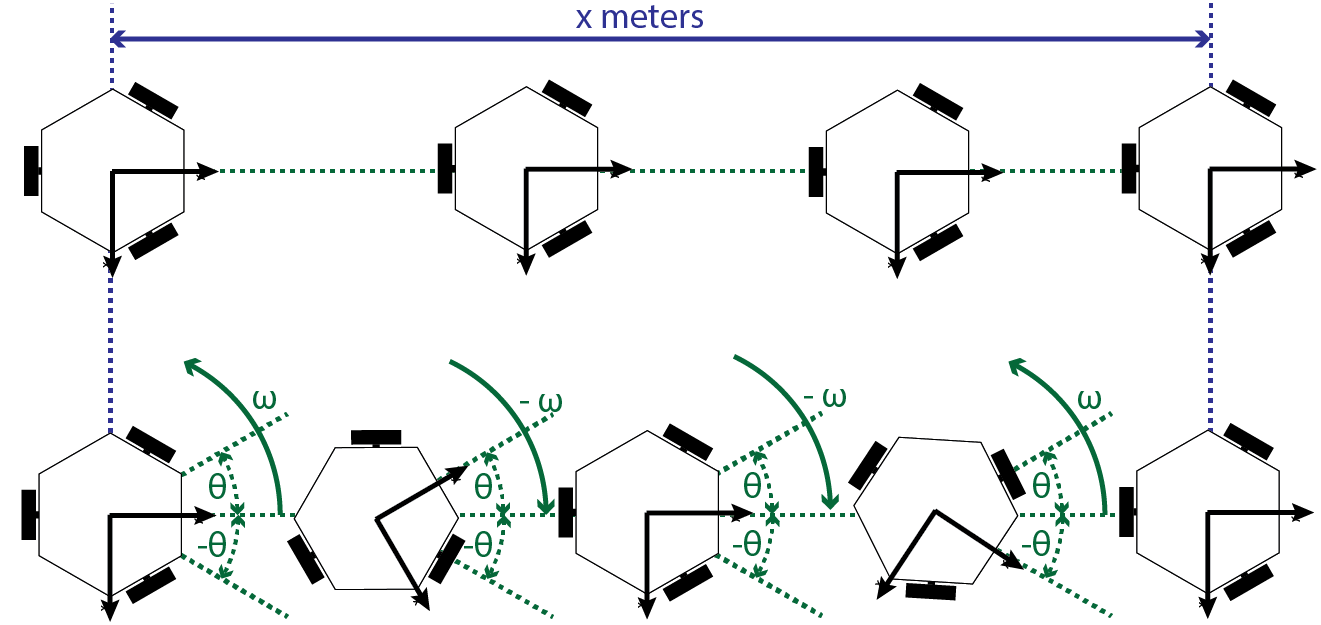
\includegraphics[width=0.75\textwidth]{./Images/ExampleMovement.png}
	\caption{Example applying the features used in all case studies. $x$ represents the displacement in meters, $\omega$ is the angular velocity ($rad/s$) and $\theta$ the oscillation of the body around its center ($rad$). The upper sequence depicts a movement based only on linear velocity, while the bottom one shows a sequence with both angular and linear movement.}
	\label{fig:features}
\end{figure} 


\section{First Case Study: Empirical Emotion Parameters}

With our first version of the platform (Figure~\ref{fig:triskar-first-design}), we decided to do our first case study at the Museum of Science and Technology in Milan, where high school students and families were coming for an event that lasted 4 days. 

%%%%%%%%%%%%%%%%%%%%%%%%%
%%%%%%%%%%%%%%%%%%%%%%%%%

\subsection{Experimental Design}

Each group of participants was exposed to three rounds, in each of which the robot was expressing a different emotion. The sequence of rounds was generated randomly without repeating any emotion in the same sequence. The subjects were asked to mark the emotion-related term that best described what they believed the robot was trying to express, selecting among a set of nine possible options: \textit{anger}, \textit{curiosity}, \textit{disgust}, \textit{embarrassment}, \textit{fear}, \textit{happiness}, \textit{sadness}, \textit{pride}, and \textit{neutral}. The option to answer ``Unknown'' was also included. Although these ten options were enlisted, just the first eight emotions were implemented. To avoid that spectators could be influenced by previous trials, different emotions were shown to each group.

Additionally, every time that a new emotion was showed, the robot started $1.5 m$ away from the participants, with its front facing them, as shown in  Figure~\ref{fig:setup}. 

\begin{figure}[h]
	\centering
	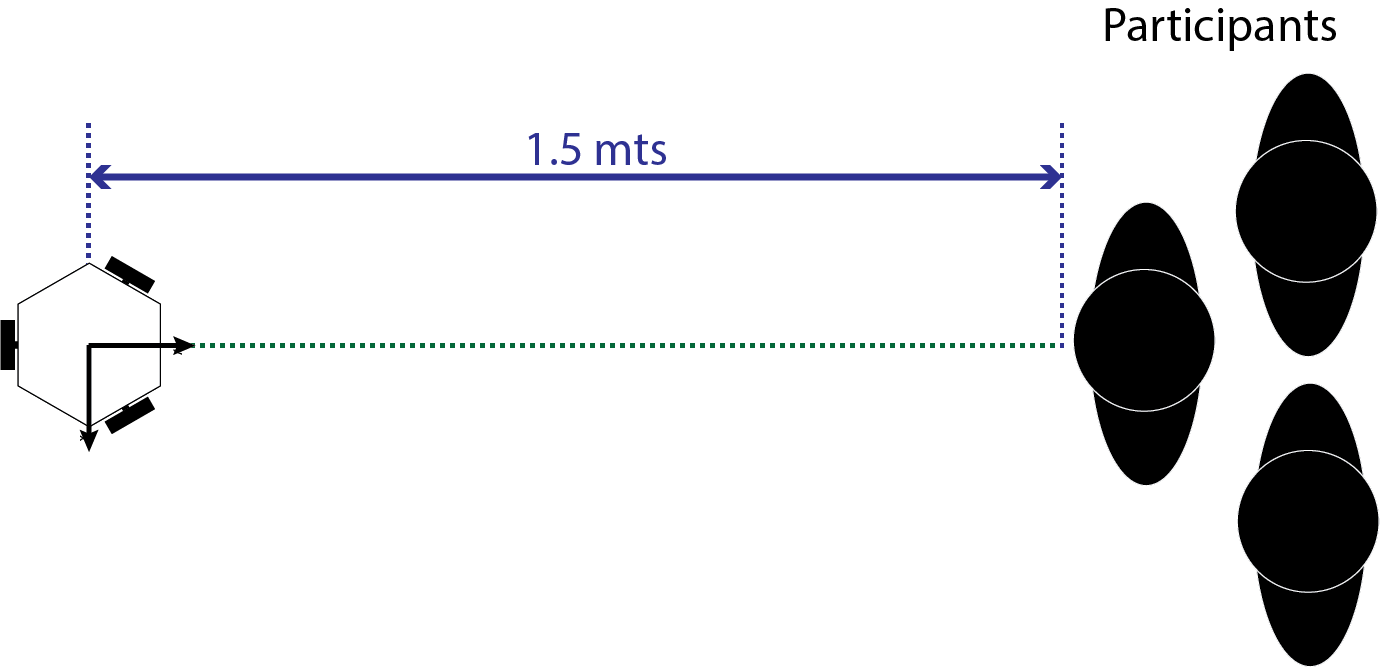
\includegraphics[width=0.7\textwidth]{./Images/FirstCase.png} 
	\caption{First case study setup.}
	\label{fig:setup}
\end{figure}  

%%%%%%%%%%%%%%%%%%%%%%%%%
%%%%%%%%%%%%%%%%%%%%%%%%%

\subsection{Emotion Description}

It was decided to follow an empirical design for this case study, by considering features that could be changed in the robot base and by composing them to express some basic emotions. The first implementations were tested and tuned basing on the emotions perceived by us from the robot's movement. The features that could be easily perceived are summarized in table~\ref{table:features}, and each selected feature is described here below:

\begin{itemize}

	\item \textit{Speed} is the target speed for the robot during the movement. It could take one out of five values: very slow (100 mm/s), slow (200 $mm/s$), normal slow (300 $mm/s$), normal (400 $mm/s$), and fast (800 $mm/s$).

	\item \textit{Front/Back} represents the fact that the robot moves backwards at some point in its movement, before going forward again; the possible values are: ''yes1``, which means that the robot goes back only once, ''yes2`` when the robot goes back twice, and ''no`` if the robot goes only forward.

	\item \textit{Shoulder} considers the movement of the upper part: ''asymmetric`` when the two beams move asymmetrically, alternatively, one forward, and the other backward, ''close``, when the upper parts get close to each other, a combination of the two (''close-2``), and ''none``. 

	\item \textit{Shoulder Amplitude} is the maximum angle that the two beams have to rotate. There are five possibilities: ''none`` ($0^\circ$), ''small`` ($10^\circ$), ''medium`` ($30^\circ$), ''large`` ($50^\circ$), and ''huge`` ($70^\circ$).

	\item \textit{Angular Velocity} $\omega$ is classified as: ''none`` (0 $mm/s$), ''slow`` (300 $mm/s$), ''medium`` (500 $mm/s$), and ''fast`` (800 $mm/s$).

	\item \textit{Body Rotation Amplitude} is the maximum  rotation angle around its center that the robot base can reach during the linear movement (it is a holonomic base); it could be: ''none`` ($0$) rad, ''small`` ($0.1$) rad, ''medium`` ($0.3$) rad, ''large`` ($0.5$) rad, and ''huge`` ($0.7$) rad.
\end{itemize}

\begin{table}[tbh]
\begin{center}
\small
\caption{Features that were presented in the first case study to the audience, and their respective values. Embarr. is Embarrassment and Asy. is Asymmetric.}
\label{table:features}
\begin{tabular}{|p{1.5 cm}|p{1.5 cm}|c|p{1.5 cm}|p{1.6 cm}|p{1.6 cm}|m{1.5 cm}|}
\hline 
\textbf{Emotion} & \textbf{Speed} & \textbf{Front/Back} & \textbf{Shoulder} & \textbf{Shoulder Amplitude} & \textbf{Angular Velocity} & \textbf{Body Rotation Amplitude} \\ 
\hline
Anger & Fast & No & Asy. & Medium & None & Very Small \\
\hline
Sadness & Very Slow & Yes-1 & Close-2 & None & Slow & Small \\
\hline
Fear & Normal Slow & Yes-2 & Close-2 + Asy. & Small & None & None \\ 
\hline
Embarr. & Slow & No & Asy. & Large & Slow & Small \\
\hline
Happiness & Fast & No & Asy. & Medium & Fast & Small \\
\hline
Disgust & Slow & No & Few Asy. & Small & None & Very Small \\
\hline
Curiosity & Normal & No & Asy. & Medium & Slow & Large \\
\hline
Neutral & Normal & No & Asy. & Medium & None & None \\
\hline
\end{tabular}
\end{center}
\vspace{-0.5cm}
\end{table} 

%%%%%%%%%%%%%%%%%%%%%%%%%
%%%%%%%%%%%%%%%%%%%%%%%%%
\subsection{Experimental Setup}

There was no specific group size, since this was determined by the amount of people that got close to the both at a given moment. Therefore, there were groups with just one person and others with 24 persons. The total amount of volunteers was 154: 55 males, 26 females, and 73 that did not specify their gender. The average age was 21.95 with a standard deviation of 12.26, minimum age was 5, maximum 62.

\subsection{Results}

Table~\ref{table:results_1} shows the results obtained in the first case study. 
\begin{table}[tbh]
\caption{Answers obtained in the first case study. On each row is the emotion that was intended to express, and on the columns the reported emotions.}
\small
\label{table:results_1}
\centering
\begin{tabular}{|c|c|c|c|c|c|c|c|c|c|c|c|c|}
\hline
\backslashbox{Presented}{Reported} & 
\rotatebox{90}{\textbf{Anger}}&
\rotatebox{90}{\textbf{Curiosity}}&
\rotatebox{90}{\textbf{Disgust}}&
\rotatebox{90}{\textbf{Embarr.}}&
\rotatebox{90}{\textbf{Fear}}&
\rotatebox{90}{\textbf{Happiness}}&
\rotatebox{90}{\textbf{Neutral}}&
\rotatebox{90}{\textbf{Pride}}&
\rotatebox{90}{\textbf{Sadness}}&
\rotatebox{90}{\textbf{Unk.}}&
\rotatebox{90}{\textbf{Tot.}}&
\rotatebox{90}{\textbf{Percentage}}\\
\hline
Anger &23 &11 &3 &4 &7 &6 &1 &0 &0 &4 &59&38.98\%\\
\hline
Curiosity &2 &9 &3 &9 &2 &3 &2 &8 &3 &0 &41&21.95\%\\
\hline
Disgust& 1 & 11& 1& 3& 7& 3& 6& 8& 5& 1& 46&2.17\%\\
\hline
Embarr. & 3& 11& 0& 8& 9& 3& 0& 4& 2& 1& 41&19.51\%\\
\hline
Fear & 3& 29& 5& 25& 22& 2& 2& 0& 2& 2& 92&22.82\%\\
\hline
Happiness & 15& 4& 0& 2& 3& 28& 4& 4& 2& 1& 63&44.44\%\\
\hline
Neutral & 5& 0& 1& 1& 0& 1& 0& 3& 2& 0& 13&0\%\\
\hline
Sadness & 4& 5& 1& 11& 13& 0& 2& 3& 7& 0& 46&23.81\%\\
\hline
\end{tabular}
\end{table}

Table~\ref{table:results_1} shows that the best emotion perceived was \textit{happiness} and the worst one \textit{disgust}, with 44\% and 2\% respectively of accuracy. Moreover, some movements were designed to convey a specific emotion, but a different emotion was perceived. For example the intended \textit{sadness} was identified by 14\% of subjects exposed to it, while 25.5\% perceived it as \textit{fear}. The neutral behaviour was not much considered, possibly because people, in this setting, expected to see something specific, not a neutral movement. To analyse whether each emotional expression was misinterpreted with others a Fisher's exact test was applied for each implemented combination of emotions. Additionally, a Holm-Bonferroni correction was applied for multiple comparisons to get better p-value estimation. 
The results showed that people perceived the following implementations as similar, having a $p-value>0.05$: \textit{curiosity-disgust}, \textit{curiosity-embarrassment}, \textit{curiosity-sadness}, \textit{disgust-embarrassment}, \textit{disgust-sadnes}s, \textit{embarrassment-fear}, \textit{embarrassment-sadness}, and \textit{fear-sadness}. 

Moreover, an analysis was done per groups, for each presented emotion. Excluding unknown and uncertain answers, we have considered the answers of each subject to whom an emotion produced by the robot was presented. For each emotion we considered how many subjects in each group recognized it, how many identified a different emotion, how many identified the considered emotion when presented another one (in any of the other two experiences each did), and how many recognized an emotion different from the considered one when presented a different emotion. This lead to a table for each presented emotion, like the one reported in Table~\ref{table:singleEmotion} for \textit{happiness}. 

\begin{table}[h]
\begin{center}
\small
\caption{Example of table compiled for each emotion on the subjects that have been presented each emotion (here \textit{happiness} for the first case study).}
\label{table:singleEmotion}
\begin{tabular}{|c|c|c|}
\hline 
\backslashbox{Presented}{Reported}&Happiness&Other\\
\hline 
Happiness&28&4\\
\hline 
Other&30&96\\
\hline
\end{tabular}
\end{center}
%\vspace{-0.5cm}
\end{table}

For each of these tables the classification accuracy and the no-information rate (NIR), i.e., the accuracy that had been obtained by random selection, have been computed with the R package CARET~\cite{caret}.
The results show that some implementations of emotion expression (i.e., \textit{anger} ($p-value=1e-3$) and \textit{happiness} ($p-value=2.8e-5$)) have been recognized by the respective panels, while others are not.

The result shows that it is possible to convey some emotions using just movement and a non-bio-inspired embodiment. In particular, stronger emotions have been recognized better than milder ones, and emotions typically conveyed by facial expressions (e.g., \textit{disgust}) were less recognized. 
%%%%%%%%%%%%%%%%%%%%%
\section{Second Case Study: Addition of Context}

Since the results of the first case study showed that the recognition of most of the designed emotions was still quite poor, it was decided to try again with the same emotion expressions, but this time a context to the emotional state of the robot was provided by playing a little scene. This is motivated by the fact that that emotions are triggered by stimuli~\cite{Plutchik2001,cacioppo2000handbook}.
%%%%%%%%%%%%%%%%%%%%%%%%%
%%%%%%%%%%%%%%%%%%%%%%%%%

\subsection{Experimental design}

A little scene was created for each emotion were an actor played the stimulus to trigger an emotion\footnote{The scenes could be seen following the link \url{https://www.youtube.com/watch?v=AXAglJKLwbI}}; for instance, he yelled at the robot that then showed \textit{fear}. The procedure and questionnaire were the same as those adopted for the first case. However, a variant of the \textit{fear} emotion (\textit{Fear2}) was added, in which the robot finishes its trajectory far from the person. As done in the first case, each group was exposed to three emotions and the sequence presented to each group was different to eliminate the chance to influence other groups. The sequences were generated randomly, without repeating the same emotion in a sequence.

As in the first case study, the total distance covered by the robot was $1.5 m$, but this time the robot was facing the actor, instead than the public. The distance from the participants to the scene (including robot and actor) was $1.5 m$, as shown in Figure~\ref{fig:setup2}. 

\begin{figure}[h]
	\centering
	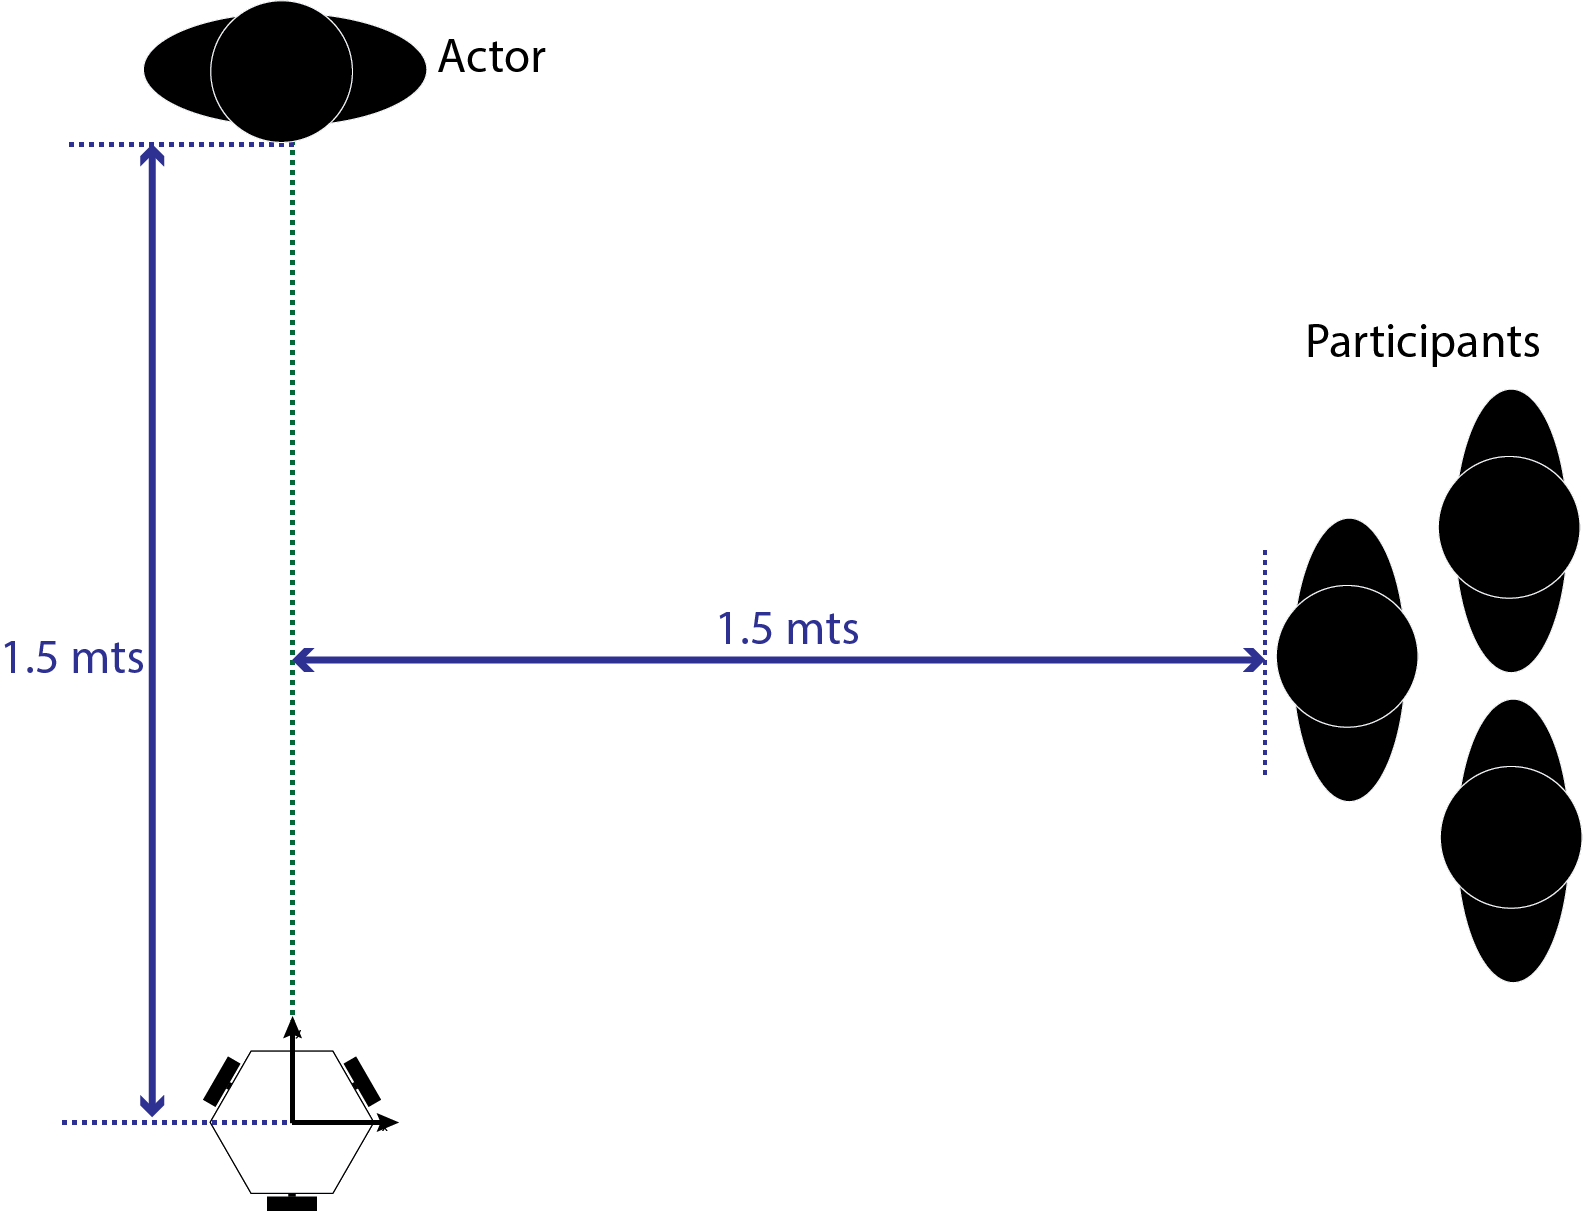
\includegraphics[width=0.6\textwidth]{./Images/SecondCase.png} 
	\caption{Setup of the second case study.}
	\label{fig:setup2}
\end{figure}
%%%%%%%%%%%%%%%%%%%%%%%%%
%%%%%%%%%%%%%%%%%%%%%%%%%
\subsection{Experimental setup}

The laboratory Open Day was used to perform the scenes and to collect data. Eight groups participated, each one with approximately 20 volunteers for a total of 156: 51 males, 17 females, and 88 that did not provide their gender. The average age was 26.34 with a standard deviation of 12.44, and with a minimum age of 11 and maximum of 65.

%%%%%%%%%%%%%%%%%%%%%%%%%
%%%%%%%%%%%%%%%%%%%%%%%%%
\subsection{Results}

Table~\ref{table:results_2} shows the results obtained in the second case study.

\begin{table}[tbh]
\caption{Answers obtained in the second case studies. On each row is the emotion that was intended to express, and on the columns the reported emotions.}
\small
\label{table:results_2}
\centering
\begin{tabular}{|c|c|c|c|c|c|c|c|c|c|c|c|c|}
\hline
\backslashbox{Presented}{Reported} & 
\rotatebox{90}{\textbf{Anger}}&
\rotatebox{90}{\textbf{Curiosity}}&
\rotatebox{90}{\textbf{Disgust}}&
\rotatebox{90}{\textbf{Embarr.}}&
\rotatebox{90}{\textbf{Fear}}&
\rotatebox{90}{\textbf{Happiness}}&
\rotatebox{90}{\textbf{Neutral}}&
\rotatebox{90}{\textbf{Pride}}&
\rotatebox{90}{\textbf{Sadness}}&
\rotatebox{90}{\textbf{Unk.}}&
\rotatebox{90}{\textbf{Tot.}}&
\rotatebox{90}{\textbf{Percentage}}\\
\hline
Anger &41 &1 &2 &0 &6 &9 &0 &2 &0 &1 &62&66.13\%\\
\hline
Curiosity &8 &38 &0 &3 &0 &4 &1 &1 &1 &4 &60&63.33\%\\
\hline
Disgust& 6& 2& 5& 4& 3& 0& 4& 7& 4& 3& 38&13.16\%\\
\hline
Embarr. & 7& 2& 1& 4& 12& 0& 0& 1& 10& 0& 37&10.81\%\\
\hline
Fear & 0& 13& 0& 17& 10& 6& 0& 0& 0& 0& 46&21.74\%\\
\hline
Fear2 & 3& 0& 5& 5& 35& 0& 1& 0& 2& 0& 51&68.63\%\\
\hline
Happiness & 0& 1& 0& 0& 5& 55& 1& 0& 0& 1& 63&87.30\%\\
\hline
Neutral & 1& 3& 2& 5& 7& 9& 5& 5& 1& 1& 39&12.82\%\\
\hline
Sadness & 0& 4& 2& 22& 14& 0& 2& 3& 15& 1& 63&23.81\%\\
\hline
\end{tabular}
\end{table}

In this second case study, the results were considerably better: four out of the nine showed emotion representations had a recognition percentage higher than 60\% (\textit{Anger}, \textit{Happiness}, \textit{Curiosity} and \textit{Fear2}). Another important point to highlight is that \textit{Sadness}, \textit{Fear} and \textit{Embarrassment} were still perceived as different emotions. As it was done for the first case study, a Fisher's exact test and Holm-Bonferroni correction were applied for each possible combination of implemented emotions. The results suggest that no implementation was considered as similar by the participants, since for all we have $p-value<(\alpha = 0.05)$. 
Comparing the percentage from both the first two cases, it is possible to see that giving information about the context that produces the current emotional state of the robot improves the recognition of some emotions, but for others remains still low. Our hypothesis is that there must be a match between robot's movements with the given context and actor's performance to increase the recognition rate. If one or both do not fit participants' idea of the emotion, this one is not going to be recognized. To verify this, a comparison between the results obtained for each emotion in both cases doing a Fisher's exact test was done. The results suggest that implementations of \textit{Disgust} ($p=0.088$), \textit{Fear} ($p=0.206$) and \textit{Sadness} ($p=0.269$) are perceived as the same in both cases, which correspond to the emotions with lower recognition rate. This opens the question about the influence that could have the human actor and the scene on the recognition rate. Although the study of this could be beneficial, it was decided to leave this to future work. Instead, a third case study was devised, where values presented in the literature for emotion expression in humans were adopted in the quest for more recognizable emotion expressions.

%%%%%%%%%%%%%%%%%%%%%
\section{Third Case Study: Literature Emotional Parameters}

The third case study was designed to explore the possibility to adopt for robot's movements the emotional movement descriptions reported in human body studies. The methodology used by Sharma and collaborators~\cite{Sharma2013} was adopted to select the emotions to be implemented and enlisted in the questionnaire. The second version of the platform was used in this case study (Figure~\ref{fig:triskar-second-design}).

%%%%%%%%%%%%%%%%%%%%%%%%%
%%%%%%%%%%%%%%%%%%%%%%%%%
\subsection{Experimental design}

In order to reduce the number of possible sequences, it was decided to implemented only four emotions. To select the emotions to be implemented, the \textit{circumplex model of affect} was adopted, as it was suggested by Sharma. The implemented emotions were: \textit{Happiness} (I quadrant), \textit{Anger} (II quadrant), \textit{Sadness} (III quadrant), and \textit{Content} (IV quadrant). To reduce the probability that the correct emotion could be selected by chance, four additional emotions were selected following the same selection procedure of the implemented ones, one from each quadrant. These emotions were: \textit{Frustration}, \textit{Boredom}, \textit{Astonishment}, and \textit{Tiredness}. The final questionnaire had nine possibilities (eight emotions and ``Unknown''), and was better founded on psychological theory than the previous ones. 

In order to study the influence that could be generated by the given list of emotions to the participants, it was presented, to another set of subjects, an open questionnaire that did not list any emotion, but rather had a space where they could write a term to answer the question: "\textit{What emotion has the robot expressed?}".
The setup used in this case study is depicted in Figure~\ref{fig:setup2}.

\begin{figure}[h]
	\centering
	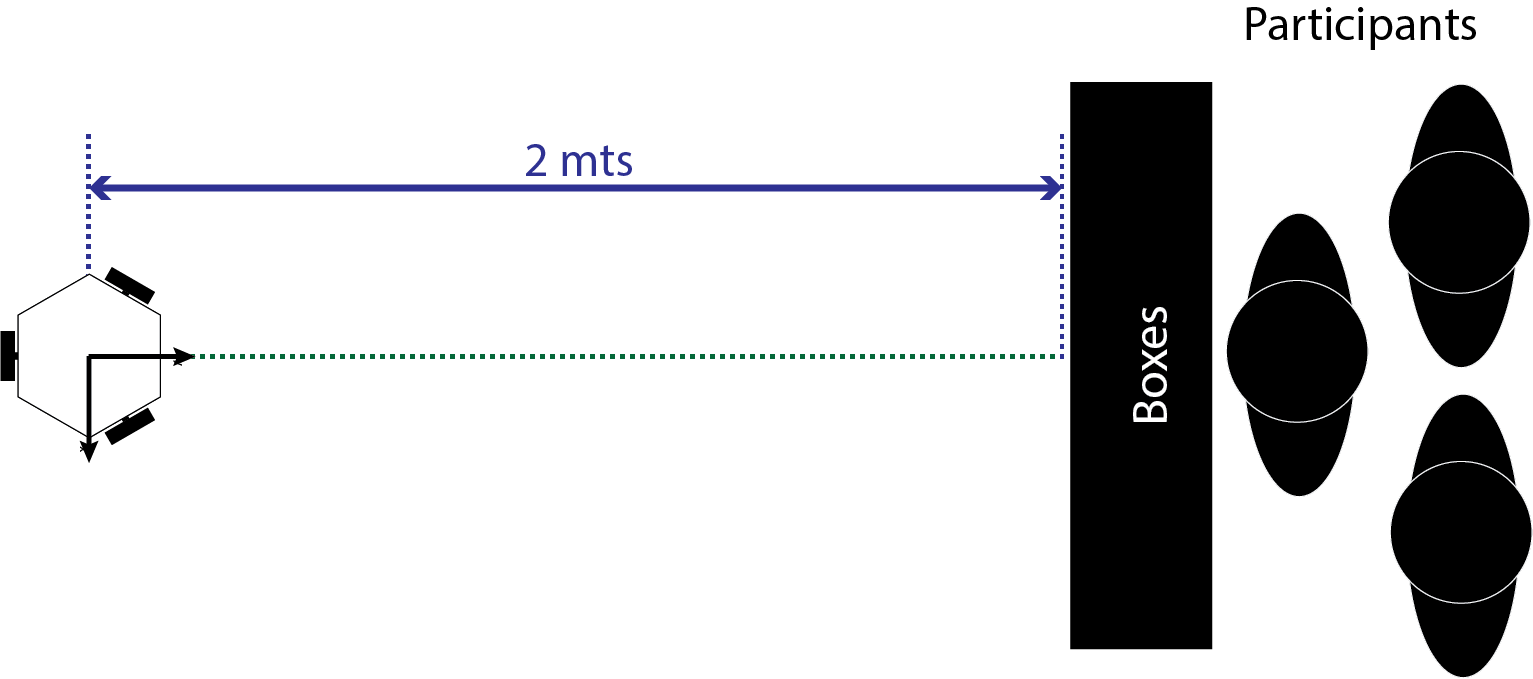
\includegraphics[width=0.6\textwidth]{./Images/ThirdCase.png} 
	\caption{Setup of the third case study.}
	\label{fig:setup2} 
\end{figure}

%%%%%%%%%%%%%%%%%%%%%%%%%
%%%%%%%%%%%%%%%%%%%%%%%%%
\subsection{Emotion Description} 

Due to the scarce literature about emotional parameters in robotics, the selection of the parameters for the implemented emotions were made following the literature in human emotion projection~\cite{Nadia2013, Crane2013}.
Generally speaking, these works use the Laban's model to code their emotional expressions, which is based on linguistic terms and leaves to the designer their specific interpretation.

The specific values selected for each emotion are reported as follow:

\begin{itemize}
	
	\item \textit{Anger}: the strong force required by Laban was interpreted as a high speed and then a sudden drop, thus it was decided to have a velocity of $500mm/sec$ for $50mm$ and then a velocity of $300mm/sec$. An oscillation during the whole trajectory was also added; that was between [0.086, -0.086] radians with an angular velocity of $3.5 rad/sec$.
	
	\item \textit{Happiness}: as in \textit{Anger}, for the first $50mm$ the velocity was $500mm/sec$, then it went down to $400mm/sec$ for another $50mm$, and then up again to $800mm/sec$ for the rest of the movement. 
	An oscillation between [0.26, -0.26] radians with an angular velocity of $3rad/sec$ was also added.
	
	\item \textit{Sadness}: the required "low energy" was interpreted as low speed and then slowing down the pace, thus a velocity of $150mm/sec$ was used for the first $200mm$, a velocity $250mm/sec$ for the next $200mm$, and for the rest a velocity of $300mm/sec$. This emotion expression did not include any angular rotation.
	
	\item \textit{Content}: the velocity was $150mm/sec$ for the first $200mm$, then $300mm/sec$ for the rest. The maximum and minimum angle of oscillation were [0.175, -0.175] with angular velocity of $0.17rad/sec$
\end{itemize}

It is important to notice that these parameters do not include any changes in the upper part of the body, since the changes done in the platform significantly decreased the emotion expression of the upper part.

%%%%%%%%%%%%%%%%%%%%%%%%%
%%%%%%%%%%%%%%%%%%%%%%%%%
\subsection{Experimental setup}

This case study was done during the Rome Maker Faire, 2014. During a period of four days, people were asked to participate to this study. Each subject was exposed to two rounds: in each one, the robot was performing a different emotion. During the first two days, the open questionnaire was used, while during the last two days the multiple option questionnaire was used. The total number of volunteers for the closed list questionnaire was 91: 52 males, 38 females, and 11 that did not specify their gender. The average age was 30.98 years, with standard deviation of 15.12, minimum age was 4 and maximum 71. The total amount of participants assessing the study with the open questionnaire was 84: 47 males, 36 females, and 1 that did not specify; the average age was 24 years, with standard deviation of 15.8, minimum age was 5 and maximum 59. 

%%%%%%%%%%%%%%%%%%%%%%%%%
%%%%%%%%%%%%%%%%%%%%%%%%%
\subsection{Results}

From the open questionnaire, different terms to describe both emotions and mental states were obtained. The results are reported in table~\ref{table:open_questionnaire}. In order to reduce the quantity of terms, words that have a similar meaning were grouped, for example words such as Fear, Terror, Scared, and Worried were grouped under the label \textit{Fear}. Also, three out of four emotions (\textit{Anger}, \textit{Happiness} and \textit{Sadness}) were at least once listed correctly. \textit{Sadness} and \textit{Content} were mostly perceived as \textit{Fear}, being reported 31\% and 28\% of the time, respectively.

From these results two important facts emerge.

\begin{itemize}
	
	\item Language richness to refer to emotions and the vague definition of emotions let people to use words that could not be directly associated to a specific emotion. 
	
	\item Movements that could be designed as emotional are also associated to mental states attributed to the robot. This is evident in the words obtained from the presentation of four ``emotional'' movements, such as: cold (referring that the robot was feeling cold), tenderness, shyness, power, hurry, looking for something, he wants something, enthusiasm, sympathy, vanity, and obedience. 
	
\end{itemize}

%%%%%%%%%%%%%%%%%%%%%%%%%%%
\begin{table}[h]
\centering
		\caption{Results obtained from the open questionnaire in the third case study.}
		\label{table:open_questionnaire}
		\small
			\begin{tabular}{|c|c|c|c|c|c|}
				\hline
					\backslashbox{Presented}{Reported}&Anger&Happiness&Sadness&Content&Total\\
				\hline
					Anger& 3&6&7&5&21\\
				\hline
					Happiness&12& 18&0&6&36\\
				\hline
					Sadness&0&0& 8&3&11\\
				\hline
					Content&2&0&0& 0&2\\
				\hline
					Fear&4&5&14&13&36\\
				\hline
					Tiredness&1&0&1&1&3\\
				\hline
					Cold&2&0&2&1&5\\
				\hline
					Shyness&1&0&4&4&9\\
				\hline
					Agitated&4&1&0&0&5\\
				\hline
					Power&4&1&0&0&5\\
				\hline
					Hurry&0&1&0&0&1\\
				\hline
					Looking for something&1&0&1&0&2\\
				\hline
					He wants something&1&0&1&0&2\\
				\hline
					Tenderness&1&0&1&2&4\\
				\hline
					Uncertainty&1&2&0&0&3\\
				\hline
					Enthusiasm&1&0&0&0&1\\
				\hline
					Sympathy&1&0&2&4&7\\
				\hline
					Curiosity&1&2&3&3&9\\
				\hline
					Shame&0&0&0&1&1\\
				\hline
					Nothing&1&2&1&0&4\\
				\hline
					Vanity&1&0&0&0&1\\
				\hline
					Obedience&0&0&0&1&1\\
				\hline
					Total&43&38&44&46&171\\
				\hline
			\end{tabular}
\end{table}

A summary of the obtained answers is provided in Table~\ref{table:result_list_emotions}.

\begin{table}[h]
\centering
\small
\caption{Answers obtained from the closed list group in the third case study.}
		\label{table:result_list_emotions}
		\begin{tabular}{|c|c|c|c|c|c|c|c|c|c|c|}
			\hline	
\backslashbox{Presented}{Reported}&
\rotatebox{90}{Anger}&
\rotatebox{90}{ Happiness} &
\rotatebox{90}{Sadness}&
\rotatebox{90}{Content}&
\rotatebox{90}{Frustration}&
\rotatebox{90}{Boredom}&
\rotatebox{90}{Astonishment}&
\rotatebox{90}{Tiredness}&
\rotatebox{90}{Unknown}&
\rotatebox{90}{Total}\\	
			\hline
				Anger&19&8&1&5&7&2&5&1&0&48\\
			\hline
				Happiness&18&19&0&9&5&1&5&1&0&58\\
			\hline
				Sadness&1&9&12&2&4&5&7&6&0&46\\
			\hline
				Content&2&8&7&4&6&8&5&10&0&50\\	
			\hline	
			\end{tabular}
\end{table}

An analysis was done for each emotion, therefore it was created a contingency matrix such as it was done in the first case study.
Additionally, two confusion matrices were created: one merging the results from all high (\textit{Anger}, \textit{Happiness}, \textit{Frustration} and \textit{Astonishment}) and low (\textit{Sadness}, \textit{Content}, \textit{Boredom}, and \textit{Tiredness}) arousal emotions; the other matrix merges the results of positive (\textit{Happiness}, \textit{Content}, \textit{Astonishment}, and \textit{Tiredness}) and negative (\textit{Anger}, \textit{Frustration}, \textit{Boredom}, and \textit{Sadness}) emotions. For each of these tables, the positive predictive value, accuracy and a Pearson's $\chi^2$ were calculated. The results are shown in table~\ref{table:Precision}. They show that there is significant evidence to conclude that \textit{Anger}, \textit{\textit{Happiness}}, and \textit{Sadness} could be perceived, while the implementation of \textit{Content} was not significantly recognized. Moreover, high and low arousal are perceived as different, but this is not the case for positive and negative valence. 

%%%%%%%%%%%%%%%%%%%%%%%%%%%%%%%%%%%
\begin{table}[h]
	\begin{center}
\small
		\caption{Accuracy, precision and results of Pearson's $\chi^2$ for each contingency matrix with $\alpha = 0.05$ for the third case study.} 
\label{table:Precision}
		\begin{tabular}{|p{3 cm}|p{2 cm}|c|c|c|}
		\hline
		\textbf{Presented Emotion} & \textbf{Positive Predicted Value} & \textbf{Accuracy} & \textbf{$\chi^2(1)$} & \textbf{p-value}\\
		\hline		
		High/Low Arousal & 0.81 & 0.69 & 28.7 & 8.29e-8\\
		\hline
		Positive/Negative Valence & 0.56 & 0.55 & 1.9 & 0.167\\
		\hline
		\hline
		Anger & 0.4 & 0.75&13.923 & 1.9e-4\\
		\hline
		Happiness & 0.33 & 0.68&4.88&2.7e-2\\
		\hline
		Sadness & 0.26 & 0.79&15.22&9.5e-5\\
		\hline
		Content & 0.08 & 0.69&6e-2&0.8 \\		 
		\hline
		\end{tabular}
	\end{center}
\end{table}

To analyse whether any emotion expression was misinterpreted among them, a Fisher's exact test and Holm-Bonferroni correction were applied for each possible combination of the implemented emotions, which gives a total of seven combinations.  
The results suggest that the implementations of \textit{Anger} and \textit{Happiness} ($p-value=0.9$), and, respectively, \textit{Sadness} and \textit{Content} ($p-value=0.9$) are interpreted as similar, while all the other emotion expressions are distinguished from each other. 

From the results of both questionnaires, we can say that \textit{Anger} and \textit{Happiness} were confused, as well \textit{Sadness} and \textit{Content}. \textit{Fear} was selected when the two emotions with low arousal (\textit{Sadness} and \textit{Content}) were shown. These results show that velocity plays a role to elicit emotions, but that it is necessary to add additional features (e.g., changes on body shape) to increase the discrimination among low and high arousal emotions, respectively. Having obtained similar results in the first and third case studies, we decided to design an experiment to identify values that could lead to better expressions of some emotions~\cite{Angel2017}.

%%%%%%%%%%%%%%%%%%%%%%
\section{Fourth Case Study: Experiment Cross-Validation}

After the first and third case studies, it was evident the necessity to better understand how the characteristics are related with each other and how they can be used to convey emotions. Therefore, it was decided to perform an experiment~\cite{Angel2017} to get a better insight on the contribution of angular and linear velocity, angle of oscillation, direction and orientation. To cross-validate the data collected in this experiment, we decided to do a final case study.

%%%%%%%%%%%%%%%%%%%%%%%%%
%%%%%%%%%%%%%%%%%%%%%%%%%
\subsection{Experimental design}

From the results obtained on our experiments, we selected two emotion implementations with the higher Krippendorff's alpha coefficient~\cite{Klaus2007} and mean for each emotion studied in an experiment done after the third case study. As in the previous case studies, a questionnaire was used. This time, the emotions listed in the questionnaire were the same used during the experiment: \textit{Anger}, \textit{Fear}, \textit{Sadness}, and \textit{Happiness}. Moreover, two mental states were added: \textit{Excited} and \textit{Tender}, which correspond to high and low arousal, respectively. As it was done in the previous cases, the questionnaire included the option ''unknown''. Although the platform used was the last version (Figure~\ref{fig:triskar-third-design}), the upper part was cut off to allow comparisons with the platform used in the other experiments. The case study set up could be seen in Figure~\ref{fig:setup_fourth}.

\begin{figure}[h]
	\centering
	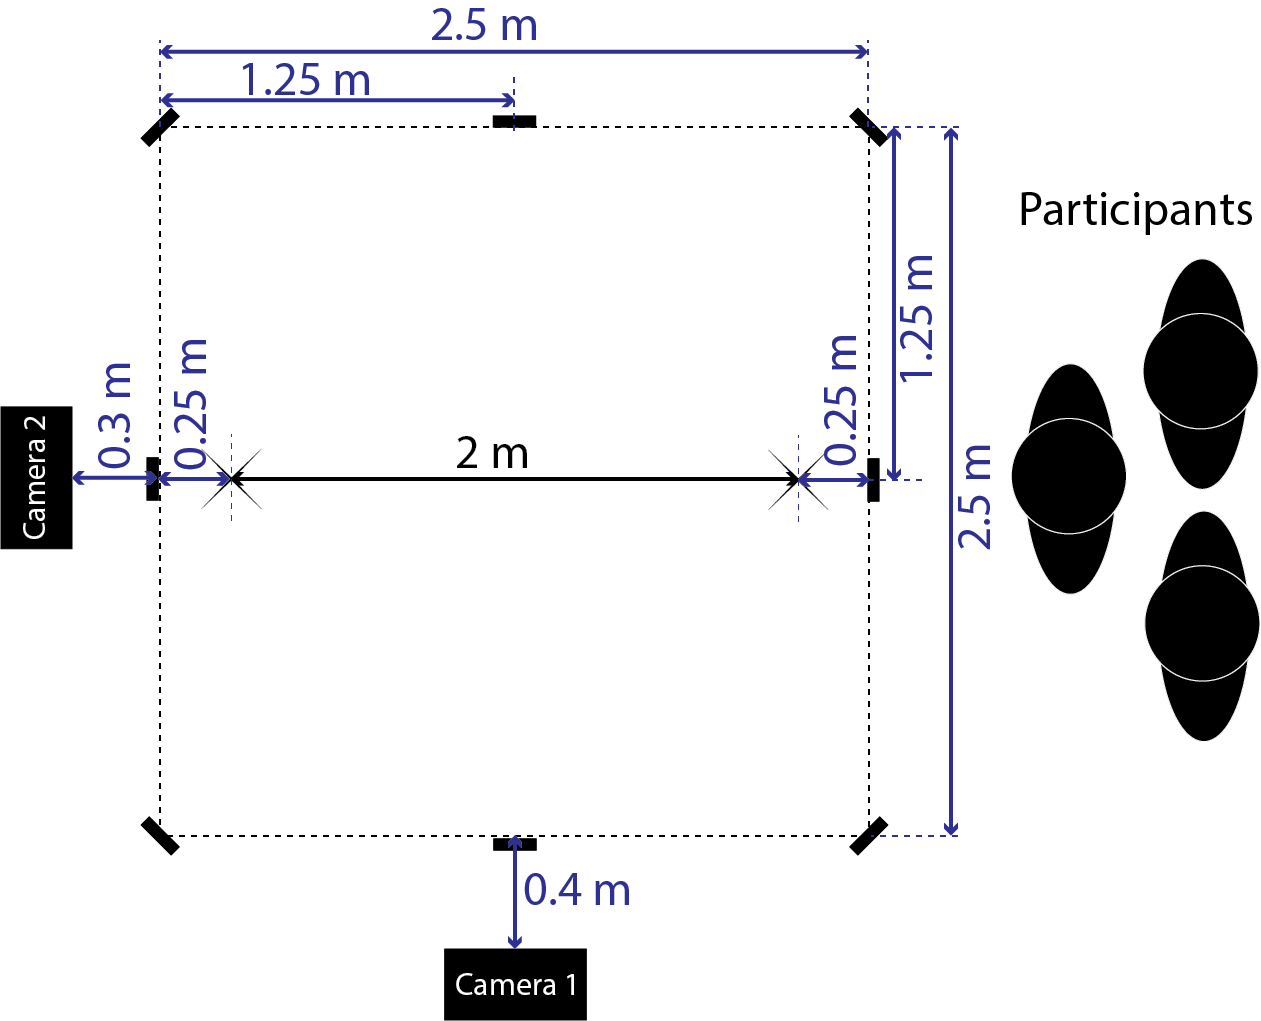
\includegraphics[width=0.60\textwidth]{./Images/FourthCase.png} 
	\caption{Environment setup for the fourth case study. The crosses symbolize the two possible starting points.}
	\label{fig:setup_fourth}
\end{figure}
 
%%%%%%%%%%%%%%%%%%%%%%%%%
%%%%%%%%%%%%%%%%%%%%%%%%%
\subsection{Emotion Descriptions} 

The parameter's values for the selected emotions are presented in Table~\ref{table:features_2}.
\begin{table}[tbh]
\begin{center}
\caption{Combination of features selected for the fourth case study.}
\label{table:features_2}
\small
\begin{tabular}{|c|c|p{2.5 cm}|p{2 cm}|p{2 cm}|p{2.5cm}|}
\hline 
\textbf{Emotion} & \textbf{Direction} & \textbf{Orientation} & \textbf{Linear Velocity} $mm/sec$& \textbf{Angular Velocity} $rad/sec$& \textbf{Oscillation Angle} $rad$\\
\hline
Happiness 1 & Getting close & Looking at the person & $500$  & $3$ & $0.349$ \\
\hline
Happiness 2 & Getting close & Looking at the person & $900$ & $3$ & $0.174$ \\
\hline
Fear 1 & Getting far & Looking at the person & $900$ & $2$ & $0.174$ \\
\hline
Fear 2 & Getting far & Looking at the person & $500$ & $2$ & $0.087$ \\
\hline
Angry 1 & Getting far & Giving the back & $500$ & $3$ & $0.087$ \\
\hline
Angry 2 & Getting close & Looking at the person & $900$ & $1$ & $0.087$ \\
\hline
Sadness 1 & Getting far & Giving the back & $200$ & $1$ & $0.349$ \\
\hline
Sadness 2 & Getting close & Giving the back & $200$ & $1$  & $0.349$ \\
\hline
\end{tabular}
\end{center}
\end{table} 

%%%%%%%%%%%%%%%%%%%%%%%%%
%%%%%%%%%%%%%%%%%%%%%%%%%
\subsection{Experimental setup}

This case study was done during the 2015 Researchers' Night. During a period of two days, people were asked to participate to this study. As in the third case study, each participant was exposed to only two emotions. The emotion sequences presented to the participants were established before hand, and randomized. The total number of participants was 256: 128 males, 126 females, and 2 unknown. The average age was 27.29 years, with standard deviation of 16.5, minimum age was 4 and maximum 76. 

%%%%%%%%%%%%%%%%%%%%%%%%%
%%%%%%%%%%%%%%%%%%%%%%%%%
\subsection{Results}

Table~\ref{table:result_fourth} summarizes the results obtained from this fourth case study.

\begin{table}[h]
\centering
\small
\caption{Summary of the answers obtained in the fourth case study.}
		\label{table:result_fourth}
		\begin{tabular}{|c|c|c|c|c|c|c|c|c|c|}
			\hline	
\rotatebox{90}{\textbf{Presented/Reported } }&
\rotatebox{90}{\textbf{Happiness}}&
\rotatebox{90}{ \textbf{Anger}} &
\rotatebox{90}{\textbf{Fear}}&
\rotatebox{90}{\textbf{Sadness}}&
\rotatebox{90}{\textbf{Excitement}}&
\rotatebox{90}{\textbf{Tenderness}}&
\rotatebox{90}{\textbf{Other}}&
\rotatebox{90}{\textbf{Total}}&
\rotatebox{90}{\textbf{Percentage}}\\	
			\hline
			Happiness 1&8&16&7&4&16&4&7&62&13\%\\
			\hline
			Happiness 2&11&11&6&2&19&3&1&53&21\%\\
			\hline
			Anger 1&7&5&6&2&21&7&1&49&10\%\\
			\hline
			Anger 2&14&29&13&2&13&3&2&76&38\%\\
			\hline
			Fear 1&6&2&28&1&9&6&0&52&54\%\\
			\hline
			Fear 2&7&3&37&2&20&4&1&74&50\%\\
			\hline
			Sadness 1&3&5&17&14&5&16&5&65&22\%\\
			\hline
			Sadness 2&5&5&15&28&6&15&7&81&35\%\\
			\hline
			\end{tabular}
\end{table} 

It could be observed that both implementations of \textit{Happiness} are confused with \textit{Anger} and \textit{Excitement}, as it could have been expected. The first implementation of \textit{Anger} was recognized as \textit{Anger} just 10\% of the times, but it was confused as \textit{Excitement} 42\%. On the other hand, the second implementation showed an improvement from 10\% to 38\% on recognition. 
This implementation was perceived also as \textit{Happiness}, \textit{Fear} and \textit{Excitement} by 18\%, 17\%, and 17\%, respectively. Both implementations of \textit{Fear} have a high level of recognition 54\% and 50\% and are mostly confused with \textit{Excitement}, 17\% for the first implementation and 27\% for the second implementation. Lastly, the first implementation of \textit{Sadness} was confused with \textit{Fear} and \textit{Tenderness} by 26\% and 24\%, respectively. The second implementation was confused again with \textit{Fear} and \textit{Tenderness} by 19\% and 19\%, respectively. 

To verify these misinterpretations among the implemented emotions, a Fisher's exact test and Holm-Bonferroni correction were applied to 10 different combinations. The results are shown in Table~\ref{table:result_compare_fourth}. As results suggest, two implementations of \textit{Anger} are the only ones that were considered as different from all others.

\begin{table}[h]
\centering
\small
\caption{Pairwise comparison among all the implemented emotions using Fisher's exact test for both questionnaires with $\alpha = 0.05$ for the fourth case study. The * indicates that the p-value was adjusted using the Holm-Bonferroni correction for multiple comparisons.}
		\label{table:result_compare_fourth}
		\begin{tabular}{|c|c|c|}
			\hline	
\textbf{Pair Compared} & \textbf{p-value} & \textbf{p-value*}\\	
			\hline
			Happiness 1 vs Happiness 2 &0.38&1.0\\
			\hline
			Anger 1 vs Anger 2 & 7.3e-4&4.4e-3\\
			\hline
			Anger 2 vs Happiness 1 & 0.137&0.69\\
			\hline
			Anger 2 vs Happiness 2 & 0.157&0.69\\
			\hline
			Fear 1 vs Fear 2 & 0.74&1.0\\
			\hline
			Sadness 1 vs Sadness 2 & 0.665&1.0\\
			\hline
			Fear 1 vs Sadness 1& 8.35e-5&5.8e-4\\
			\hline
			Fear 1 vs Sadness 2 & 5e-7&4e-6\\
			\hline
			Fear 2 vs Sadness 1 & 2e-7&1.8e-6\\
			\hline
			Fear 2 vs Sadness 2 & 1e-7&1e-6\\
			\hline
			\end{tabular}
\end{table}
 
As it was done in the previous case studies a contingency matrix was computed for each emotion. 
For each of these tables, the positive predictive value, accuracy and a Pearson's $\chi^2$ were calculated. The results are shown in table~\ref{table:Precision2}. They show that there is significant evidence to conclude that one implementation of \textit{Anger}, and both those of \textit{Fear} and \textit{Sadness} could be perceived correctly, while both implementations of \textit{Happiness} and the other one of \textit{Anger} were not.

\clearpage
\begin{table}[h]
\centering
\small
\caption{Accuracy, precision and results of Pearson's $\chi^2$ for each contingency matrix with $\alpha = 0.05$ for the fourth case study.} 
\label{table:Precision2}
		\begin{tabular}{|p{3 cm}|p{2 cm}|c|c|c|}
		\hline
		\textbf{Presented Emotion} & \textbf{Positive Predicted Value} & \textbf{Accuracy} & \textbf{$\chi^2(1)$} & \textbf{p-value}\\
		\hline
		Happiness 1 & 0.13 & 0.79 & 0.11 & 0.74\\
		\hline
		Happiness 2 & 0.21 & 0.81& 3.7 &0.054\\
		\hline
		Anger 1 & 0.1 & 0.8 & 3.8e-29 & 1\\
		\hline
		Anger 2 & 0.38 & 0.81 & 34.4 & 4.47e-9\\
		\hline
		Fear 1 & 0.54 & 0.8 & 36.2 & 1.8-e9\\
		\hline 
		Fear 2 & 0.5 & 0.78 & 35.8 & 5.3e-10\\
		\hline
		Sadness 1 & 0.22 & 0.85 & 27.4 & 1.63e-7\\
		\hline
		Sadness 2 & 0.35 & 0.85 & 72.9 & 2.2e-16\\		 
		\hline
			\end{tabular}
\end{table}
 
It is important to notice that the results were obtained using the lower part of the robot without any change in shape. Another factor to consider is the high impact that the terms enlisted in the questionnaire had in the detection rate. These terms included two mental states that could be confused with the other four emotions enlisted, as it is reflected in the results. Despite the bias generated by these two terms, the recognition rates for five over eight emotion expressions were over 35\%, being the two implementations of Fear the ones with the highest recognition rate (54\% for the first and 50\% for the second).
\section{Conclusions and Further Work}
Four case studies were done to study the contribution of angular velocity, linear velocity, oscillation angle, and shape change in emotion expression from a non-bio-inspired robot. The results collected during all case studies show that a correct combination of linear and angular velocity, oscillation angle, and direction can be used to convey emotions that could be distinguished from each other. Also, they suggest that it is necessary to modify the robot's shape to increase people's emotion recognition rate. This result is congruent with the results obtained in the studies done to understand what features are more relevant when humans convey emotions~\cite{Roether2009,Venture2014}.\\
The lessons learned after these four case studies can be summarized as:
\begin{itemize}
	\item It is possible to convey emotions through changes in angular and linear velocity of a non-bio-inspired body also without changes in the body shape. This lesson opens the door to the inclusion of simple "emotion" to robotic platforms that are not required to have bio-inspired characteristics, but have to interact with humans.
	\item The change in the body shape increases the emotion identification rate of the observers. However, the characteristics that should be changed to increment the emotions perception are still to be investigated.
	\item Although Laban's notation is adequate to code people's movements, robots need precise values to define their actions. As a consequence, the Laban's theory needs to be instantiated to the robots' situation, to enable comparison between different works.
	\item Emotions come as a reaction to an event. Therefore, just showing uncorrelated movements to the participants is not going to support the study of the expression of all the emotions. For example, the action Fear was well perceived by the participants when the robot get far from them, as they were inducing it.
	\item Giving the participants the possibility to write their interpretation of the robot's movements was not going to be helpful to assess what emotion they thought the robot was conveying during case studies. Although there are plenty of procedures that have been proposed to determine the emotion that a person could be thinking at (e.g., SAM), they could just be used in a controlled environment where the experimenter could spend long periods of time with the participant. This is not the case of exhibitions where people would agree to stop just for a couple of minutes. On the other side, exhibitions make it possible to collect a large number of subjects representative of a varied population.
	\item Using a real platform to perform the case studies increases the enthusiasms of the participants and possibly their willingness to participate in the study. Although we did not evaluate directly this item during our case studies, it was observed during the set up that people were curious to see the robot moving. Also, during the pilot two kids had a different reaction when the robot was getting close to them. One of them was scared of the robot, while the other was curious about the robot.
\end{itemize}
Further work should be done to understand how the combination of changes in the body shape could contribute to the expression of emotions. It is also necessary to recreate a simple scene to give the context to the participants, but this time just using two robots. This will eliminate possible clues that could be given by the human actor.
\bibliographystyle{apacite}
\bibliography{Bibliography,Biblography,BibloNew}
\end{document}